\documentclass[12pt]{article}
\usepackage[utf8]{inputenc}
\usepackage{graphicx}
\usepackage[letterpaper, top = 2 in, right = 1.2in, left = 1.2 in, bottom = 1 in,  headheight=95pt, headsep=30pt]{geometry}
\usepackage{setspace}
\usepackage{titlesec}
\usepackage{fancyhdr}
\usepackage{caption}
\usepackage{tikz}
\usepackage{graphicx}
\usepackage{setspace}
\usepackage{tabularx}
\usepackage{eso-pic}
\usepackage{xcolor}
\usepackage{amsmath}
\usepackage{amssymb}
\usepackage[backend = biber, style = apa]{biblatex}
\addbibresource{references.bib}

% Customization
% Document Customization
\setlength{\parindent}{0.5 in}
\titleformat{\section}[block]{\doublespacing\bfseries\centering}{}{0pt}{}
\titleformat{\subsection}[block]{\doublespacing\bfseries}{}{0pt}{}
\titleformat{\subsubsection}[block]{\doublespacing\bfseries}{}{0pt}{}
\titleformat{\subsubsubsection}[block]{\doublespacing\bfseries}{}{0pt}{}

\newcommand{\verticallineinmargin}{
    \AddToShipoutPictureBG*{
        \AtPageLowerLeft{
            % Adjust the positions and lengths of the lines here
            \put(72,0){\line(0,1){842}}  % Left margin line
            \put(540,0){\line(0,1){842}} % Right margin line
        }
    }
}

\newcommand{\horizontallinemargin}{
    \AddToShipoutPictureBG*{
        \AtPageLowerLeft{
            \put(0, 60){\line(1, 0){700}}
            \put(0, 710){\line(1,0){700}}
            \put(0, 685){\line(1,0){700}}
            \put(0, 35){\line(1,0){700}}
        }
    }
}

% Header and Footer Customization
\pagestyle{fancy}
\fancyhf{}
\fancyhead[C]{
    \verticallineinmargin
    \horizontallinemargin
    \protect\begin{minipage}{\textwidth}
        \centering
        \includegraphics[width = 50pt]{PUPLogo.png} \\
        \vspace*{0.6 cm}
        \textbf{POLYTECHNIC UNIVERSITY OF THE PHILIPPINES}
    \end{minipage}
}
\fancyfoot[C]{\thepage}
\renewcommand{\headrulewidth}{0pt}

\begin{document}
\begin{titlepage}
    \thispagestyle{fancy}
    \fancyfoot[C]{\textcolor{white}{\thepage}}
    \centering
    \vspace*{2cm}  % Adjust vertical space from the top
    \textbf{A Comparative Study of Linear and Quadratic Discriminant Analysis of Alzheimer's Disease Occurrence Based 
    on Lifestyle Factors, Clinical Measurements, and Cognitive and Functional Assessments}
    
    \vspace*{2cm} 
    Presented to \\
    Department of Mathematics and Statistics, College of Science \\
    Polytechnic University of the Philippines - Manila

    \vspace*{2cm} 
    \normalsize
    In partial fulfillment of the requirements in \\ 
    STAT 20253: Multivariate Analysis

    \vspace*{3cm}
    By \\ [0.5 cm]
    Almer John Sta. Ines \\ [0.3 cm]
    Dencie Mae Saguano \\ [0.3 cm]
    Jerolle Nonato \\ [0.3 cm]
    Joy Ellen Mae Yangyang \\ [0.3 cm]
    Juan Raphael Pimentel \\ [0.3 cm]
    Roldan Libay Jr. 
    \vfill
    \textbf{2025}
\end{titlepage}

\begin{abstract}
    \hspace{-2cm}
    \begin{tabular}{lll}
        &&\\
        \textbf{Title} &:& A COMPARATIVE STUDY OF LINEAR AND QUADRATIC \\ 
        && DISCRIMINANT ANALYSIS OF ALZHEIMER'S DISEASE \\ 
        && OCCURRENCE BASED ON LIFESTYLE FACTORS, CLINICAL \\
        && MEASUREMENTS, AND COGNITIVE AND FUNCTIONAL \\
        && ASSESSMENTS \\
        &&\\
        \textbf{Researcher} &:& Almer John Sta. Ines \\
        && Dencie Mae Saguano \\
        && Jerolle Nonato \\
        && Joy Ellen Mae Yangyang \\
        && Juan Raphael Pimentel \\
        && Roldan Libay Jr. \\
        &&\\
        \textbf{Degree} &:& Bachelor of Science in statistics \\
        &&\\
        \textbf{Institution} &:& Polytechnic University of Philippines - Manila \\
        &&\\
        \textbf{Year} &:& 2025 \\ 
        &&\\
        \textbf{Adviser} &:& Peter John Aranas \\
        &&\\
    \end{tabular}
    \doublespacing
    \noindent

    This study aims to distinguish Alzheimer’s patients from non-Alzheimer’s patients by analyzing clinical measurements, cognitive and functional assessments, and lifestyle factors. The objectives is to identify key clinical indicators, optimizing a discriminant classification model through feature reduction, and comparing the performance of Linear Discriminant Analysis (LDA) and Quadratic Discriminant Analysis (QDA) for early AD detection. The analysis used Lasso regression and Recursive Feature Elimination (RFE) for feature selection. Results showed that cognitive assessments like the Mini-Mental State Examination (MMSE) and Activities of Daily Living (ADL) are significant indicators. QDA models outperformed LDA in classification accuracy, demonstrating superior predictive power. \\
    \noindent
    \textbf{Keywords:} \textit{Linear Discriminant Model, Quadratic Discriminant Model, Alzheimer's Disease}
\end{abstract}

% Table of Contents
\newgeometry{top=2in, bottom=1in, left=1.2in, right=1.2in}
\renewcommand{\contentsname}{TABLE OF CONTENTS}
\pagenumbering{roman}
\doublespacing
\tableofcontents

% Chapter 1
\restoregeometry

\pagenumbering{arabic}
\setcounter{page}{1}

\newpage

\section{CHAPTER I \\ THE PROBLEM AND ITS SETTING}
\doublespacing
\noindent

This chapter contains the introduction, statements of the problem, research hypothesis, 
significance of the study, scope and limitations, and definition of terms. 

% Introduction
\subsection{Introduction}
\noindent

Every three seconds, someone in the world develops dementia, adding to the more than 55 million people already 
living with the condition as of 2020 (\cite{alzint_dementia_statistics}). This number is expected to nearly double 
every 20 years, reaching 78 million in 2030 and a staggering 139 million by 2050. Alzheimer's disease (AD) the most
common cause of dementia, is a progressive brain disorder that gradually affects memory, thinking skills, and the ability
to carry out everyday tasks (\cite{AlzheimersAssociation2021}). As the prevalence of AD continues to rise, it affects people not only altering their lives 
but also placing an emotional and financial strain on families and healthcare system. Early detection is crucial as it allows for 
timely interventions, potential treatments, and better support for both patients and caregivers (\cite{Dubois2016}). However, diagnosing AD in its early stages remains challenging, 
as its symptoms often overlap with other cognitive conditions, making it difficult to distinguish from normal aging or mild cognitive impairment (\cite{Jack2018}). Understanding the key
indicators of AD can help improve early diagnosis and lead to better patient outcomes.

A study by Livingston et al. (2020) suggests that lifestyle factors, medical history, clinical measurements, and cognitive and functional assessments can provide essential insights into the
early identification of Alzheimer's disease. Lifestyle factors, such as Body Mass Index (BMI), smoking status, alcohol consumption, physical activity, diet quality, and sleep quality can impact 
the risk of developing AD (\cite{nih_healthy_lifestyle}). Additionally, certain medical conditions, including hypertension, diabetes, cardiovascular, diseases, depression, family history of AD, and
head injury have been linked to increased susceptibility to AD. Clinical measurements, particularly cardiovascular health indicators, have been increasingly recognized as significant
risk factors for the disease. Moreover, a study conducted by Leszek et al. (2020) suggests that cardiovascular diseases can contribute to the development and progression of AD by impairing blood flow to the brain
and causing inflammation (\cite{Leszek2021}). Functional assessments, which evaluate how well a person can manage daily tasks and adjust to cognitive changes, can also be an important tool in detecting early signs of AD. (\cite{sperling2011})

The effectiveness of classification models in predicting AD is crucial for developing reliable diagnostic tools. LDA and QDA are two widely used statistical techniques for classification problems. LDA assumes equal covariance structures
among groups, making it more effective when the assumption holds, while QDA relaxes this assumption, allowing for more flexibility in classification (\cite{elements_statistical_learning})

The study aims to investigate significant differences between Alzheimer's patients and Non-Alzheimer's patients concerning lifestyle factor, clinical measurements, and cognitive and functional assessments. Additionally, it seeks to identify 
substantial indicators of AD and compare the discriminative power of LDA and QDA in early prediction. By analyzing there aspects, this research contributes to the development of more accurate and efficient classification models for early AD 
diagnosis. 

\subsection{Objectives}
\noindent

The general objective of the study is to accurately discriminate Alzheimer's patients to Non-Alzheimer's patients based on their lifestyle factors, clinical measurements, and cognitive and functional assessment.

Specifically, it aims to achieve the following objectives. 

\begin{enumerate}
    \item To identify which clinical indicators can effectively discriminate Alzheimer's patients to Non-Alzheimer's patients. 
    \item To optimize a discriminant classification model through feature reduction. 
    \item To compare the discriminative power of LDA and QDA for an early prediction of AD. 
\end{enumerate}

\subsection{Statements of the Problem}
\noindent

Following the mentioned objectives, the study sought to answer the following questions. 
\begin{enumerate}
    \item Are there significant differences between Alzheimer's and Non-Alzheimer's patients in terms of:
    \begin{enumerate}
        \item Lifestyle Factors
        \item Clinical Measurements
        \item Cognitive and Functional Assessment
    \end{enumerate}
    \item What are the substantial indicators of AD? in terms of: 
    \begin{enumerate}
        \item Lifestyle Factors
        \item Clinical Measurements
        \item Cognitive and Functional Assessment
    \end{enumerate}
    \item How do the discriminative powers of LDA and QDA compare in the early prediction of AD?
\end{enumerate}

\subsection{Significance of the Study}
\noindent

This research aims to develop a classification model for the early prediction of AD by analyzing key factors such as lifestyle, clinical measures, and cognitive and functional assessments. 
The findings of this study will be significant to the following sectors: 

\textbf{Healthcare Practitioner and Neurologist}. This study will provide a data-drive approach for early AD prediction, aiding in timely intervention and personalized treatment plan. Furthermore, 
this research will enhance the understanding of the most substantial indicators of AD based on statistical multivariate models. 

\textbf{Researchers and Data Scientist}. The study will contribute to the growing field of medical data analysis by exploring the effectiveness of LDA and QDA in disease membership classification. It 
will serve as a foundation for the future studies integrating machine learning and statistical methods in healthcare analytics which will potentially lead to more advanced diagnostic tools. 

\textbf{Patients and Families}. This study will benefit them as early detection tools can help them prepare for disease management and necessary lifestyle adjustments. This will also raise awareness of the 
key lifestyle and medical factors that may contribute to the risk of AD and encourage them to have preventive measures that may delay the onset of disease.

\textbf{Public Health and Policy-Makers}. This study holds significance to the public health sector by supporting the development of data-drive healthcare policies focused on early screening and intervention
programs. The insights gained from this research can help allocate resources in AD research, prevention and treatment programs.

\subsection{Scopes and Limitations}
\noindent

This study aims to develop a classification model for early prediction of AD using LDA and QDA. It focuses on analyzing and identifying important factors such as lifestyle habits, clinical measurements, and cognitive and 
functional assessments to distinguish between Alzheimer's and Non-Alzheimer's patients. The study also compares the discriminative power of LDA and QDA in identifying substantial predictors of the disease and compares their 
classification performance. 

The dataset used in this study consists of 2,149 patient records with unique identifications ranging from 4571 to 6900. It includes demographic details, lifestyle factors, medical history, clinical measurements, cognitive and functional
assessments, symptoms, and Alzheimer's diagnosis. Since the dataset is synthetically generated and designed from educational purposes, it provides a structured and controlled environment for analysis. However, because it is not based on real patient data, 
it may not fully capture the variability and complexity of real-world medical dataset. 

Despite its strengths, the study has certain limitations. Since the dataset is synthetic and not sourced from actual medical records, the generalizability of the findings to real-world clinical settings may be restricted. Additionally, LDA and QDA rely on certain
statistical assumptions, like normality and homoscedasticity for LDA, which may affect their predictive accuracy in more complex datasets. This study also does not compare LDA and QDA with other machine learning models, limiting the analysis to just these two multivariate
techniques. 

\newpage
\section{CHAPTER II \\ REVIEW OF LITERATURE AND STUDIES}

This chapter contains all local and foreign studies that the 
researchers used to serve as a foundation of understanding
for the study. The review is organized into sections 
that highlight relevant theories, empirical studies, and 
frameworks from previous researches. 

\subsection{Alzheimer's Disease}
\noindent

Alzheimer’s disease (AD) is a progressive neurodegenerative disorder primarily affecting cognitive function, memory, and daily activities. It is the most common form of dementia, accounting for approximately 60–80\% of all dementia cases (\cite{alzheimers2024}). 
The disease is characterized pathologically by the accumulation of abnormal neuritic plaques or amyloid-beta plaques and neurofibrillary tangles in the brain, leading to neuronal damage and brain atrophy (Kumar et al., 2024). These pathological changes disrupt communication between neurons, 
resulting in cognitive decline and behavioral changes. 

The progression of Alzheimer’s disease occurs in stages, typically starting with mild cognitive impairment (MCI), followed by moderate cognitive decline, and ultimately leading to severe dementia (Alzheimer’s Association, 2024). In the early stages, individuals may experience minor memory lapses 
and difficulty in recalling recent events. As the disease progresses, individuals commonly experience multiple types of symptoms that change with time including struggle with language, reasoning, and motor functions, eventually requiring full-time care due to the loss of independence (\cite{Dubois2016}).

Several risk factors contribute to the development of Alzheimer’s disease, including genetic, environmental, and lifestyle-related factors. Age is the most significant risk factor, with the majority of cases occurring in individuals over 65 years old (\cite{Livingston2020}). Genetic predisposition, 
particularly the presence of the APOE E4 allele, has been linked to an increased risk of developing Alzheimer’s (\Cite{dibattista2016}). Their genetic mutations in APP, PSEN1, and PSEN2 genes are associated with early-onset familial Alzheimer’s disease (\cite{lanoiselee2017}). 

In addition to genetic factors, medical history plays a crucial role in Alzheimer’s risk. Conditions such as hypertension, diabetes, obesity, and cardiovascular diseases have been identified as contributing factors due to their impact on cerebrovascular health (\cite{Silva2019}). 
Furthermore, lifestyle choices such as diet, physical activity, cognitive engagement, and social interactions influence brain health and may either increase or mitigate the risk of developing Alzheimer’s (\cite{Lourida2019}). Key indicators of the disease include memory impairment, difficulty in problem-solving, confusion with time and place, mood changes, and challenges in completing familiar tasks (Alzheimer’s Association, 2024).

Early diagnosis of Alzheimer’s disease is critical for implementing timely interventions that can slow disease progression and improve patient quality of life. Early detection allows for better planning, access to treatments, and participation in clinical trials aimed at finding disease-modifying therapies (\cite{Cummings2019}). 

Advancements in diagnostic tools have made early detection more feasible. Neuroimaging techniques, such as magnetic resonance imaging (MRI) and positron emission tomography (PET), help identify structural and functional brain changes associated with Alzheimer’s (\cite{Jack2018}). Additionally, biomarkers in cerebrospinal fluid (CSF) and blood, such as amyloid-beta and tau protein levels, provide promising avenues for early diagnosis (\cite{Hansson2019}).
Cognitive assessments, including the Mini-Mental State Examination (MMSE) and Montreal Cognitive Assessment (MoCA), remain essential tools for evaluating cognitive decline in clinical settings (\cite{Jia2021}). 

The development of machine learning and statistical models, such as discriminant analysis, further enhances the potential for early Alzheimer’s prediction. These models utilize patient data to classify individuals at risk, providing valuable insights into disease progression and facilitating early interventions (\cite{Arslan2022}). 
As research continues, integrating clinical, genetic, and lifestyle data into predictive models holds promise for improving early detection and personalized treatment strategies for Alzheimer’s disease.

\subsection{Discriminant Analysis in Medical Diagnosis}
\noindent

Discriminant analysis (DA) is a powerful statistical technique used to classify subjects into categories based on predictor variables, and it has been found to have extensive applications in medical diagnosis. This method is employed to assess the accuracy of a classification system in predicting the sample into specific groups. It involves creating discriminant functions for each observation and determining a cutoff score, 
which is then utilized to categorize the sample into different groups. In the medical field, DA is especially valuable for distinguishing between healthy and diseased states or for classifying patients into various disease subtypes. The development of DA methods, such as Linear Discriminant Analysis (LDA) and Quadratic Discriminant Analysis (QDA), has enabled healthcare professionals to use these techniques for improved diagnostic accuracy (\cite{Dhamnetiya2022}). 

Discriminant analysis is grounded in statistical theory and involves the calculation of a discriminant function that assigns observations to specific groups based on their characteristics. The basic concept of LDA involves maximizing the separation between two or more groups by projecting data onto a lower-dimensional space (\cite{GeeksforGeeksLDA}). 
Mathematically, LDA computes a linear combination of features that best separates the classes. In contrast, QDA introduces a quadratic term, allowing for more flexibility in the decision boundary between classes by modeling the class-conditional densities as different covariance matrices (Di Renzo, 2024). The mathematical foundation of both techniques makes them robust for various classification tasks, with LDA generally performing well when groups have similar covariance structures, and QDA being more effective when those structures differ.

While LDA assumes that the data from each class follow a Gaussian distribution with identical covariance matrices, QDA relaxes this assumption by allowing each class to have its own covariance matrix (\cite{ScikitLearnLDAQDA}).
This flexibility allows QDA to model more complex relationships in the data and may result in higher classification accuracy when the assumption of equal covariances in LDA is violated. However, QDA is more sensitive to the number of features relative to the sample size, and it may overfit with small datasets (Nxtlive, 2023). 
Furthermore, QDA is less helpful when the number of features in a data set is moderate or high, and LDA and its variants often perform better due to their robustness against dimensionality (\cite{Wu2022}). Therefore, selecting between LDA and QDA depends on the underlying assumptions of the data and the complexity of the decision boundaries.


In medical diagnostics, discriminant analysis has been widely employed, particularly for disease classification. For example, it has been successfully used in modeling medical diagnosis on diseases such as cancer, diabetes, and heart diseases. For instance in the study of \cite{Shariatnia2022}, the methods has been successfully used in modeling the diagnosis of coronary artery diseases where it was found out that the LDA method is superior to the Quadratic Discriminant Analysis (QDA), K-Nearest Neighbor (KNN) and Logistic Regression (LR) methods 
in differentiating CAD patients and is recommended as a predictive model with acceptable accuracy, sensitivity, and specificity for the diagnosis of CAD. Another application of DA is in diabetes mellitus diagnosis. The study of \cite{Kresnawati2023} used quadratic discriminant analysis and shows that it can diagnose diabetes mellitus with high performance. Hence, by leveraging features such as age, gender, lifestyle factors, and clinical biomarkers, discriminant analysis can assist in early detection and classification of disease severity. 
In the case of cancer, specifically breast cancer in the research of \cite{Adebiyi2022}, the LDA and other classification models have been used in classification and prediction of cancer as  either benign or malignant categories, and QDA has been applied to distinguish between subtypes of diseases like Alzheimer's disease, based on complex biomarker patterns (\cite{Santos2022}). 
These applications demonstrate the utility of discriminant analysis in the medical field, as it enhances diagnostic precision and enables personalized treatment planning.



\subsection{Factors Influencing Alzheimer's Disease}
\subsubsection {Lifestyle Factors}
\noindent

Lifestyle behaviors play a vital role in maintaining cognitive health and reducing the rish of Alzheimer's disease. Engaging in regular physical activity, for instance, has been linked to a lower likelihood of cognitive decline. \cite{Dominguez2021} emphasized that aerobic
exercises not only boost brain function but can also help delay the onset of dementia. Similarly, following a healthy diet, particularly one rich in fruits, vegetables, and whole grains, like the Mediterranean diet, has been shown to enhance cognitive performance and decrease
the risk of Alzheimer's. Maintaining an active social life also contributes significantly, as frequent social interactions and participation in activities foster cognitive resilience and lower the chanves of developing dementia. (\cite{Dominguez2021})

Sleep quality and duration are emerging as important factors in Alzheimer's risk. Poor sleep habits, such as not getting enough rest or experiencing disrupted sleep, have been linked to a buildup of amylod-beta in the brain, a hallmark of Alzheimer's. \cite{Dominguez2021} highlights
that good-quality sleep is essential for brain health. It helps clear out metabolic waste products and supports memory consolidation, making it a critical part of maintaining cognitive function.

\subsubsection{Clinical Measurements}
\noindent

Recent advancements in biomarker research have greatly improved the ability to classify and detect Alzheimer's disease at an early stage. Blood-based biomarkers, such as specific microRNAs (miRNAs), are showing promise in identifying individuals at risk even before symptoms appear 
(\cite{JAMA2019}). Genetics also play a key role, with the APOE4 allele being a well-known risk factor. People who carry this variant have a higher chance of developing Alzheimer's, and integrating genetic information into classification models can enhance accuracy in predicting the
disease (\cite{JAMA2019}).

Health conditions like diabetes, heart disease, and high blood pressure have been linked to a higher risk of developing Alzheimer's disease. These issues can worsen the impact of vascular problems on brain function and may even interact with Alzheimer-related changes in the brain. Taking
steps to manage these conditions through healthy lifestyle choices and medical treatments, play a key role in lowering the overall risk of dementia (\cite{PMC2021}).

\subsubsection{Cognitive and Functional Assessment}
\noindent

Cognitive tests play a crucial role in identifying and classifying Alzheimer's disease. Standard assessments like the Mini-Mental State Examination (MMSE) and the Montreal Cognitive Assessment (MoCA) help measure cognitive function in a structured way. The results from these tests provide 
valuable insights that can improve classification models, making it easier to distinguish between healthy individuals, those with mild cognitive impairment, and those with Alzheimer's disease (\cite{PMC2021}). Functional assessment, on the other hand, focuses on understanding how well a person
can handle everyday tasks and adapt to changes in their thinking abilities. Tools like the Alzheimer's Disease Cooperative Study-Activities of Daily Living Inventory (ADCS-ADL) and the Functional Activities Questionnaire (FAQ) are often used to evaluate these abilities (\cite{Custodio2022}). Supported by
the study of \cite{cummings2017} which stated that these assessments go beyond cognitive tests, offering a more complete picture of how Alzheimer;s disease affects a person's overall functioning and quality of life.

\subsection{Detection of Alzheimer's Disease using Discriminant Models}
\noindent

Linear Discriminant Analysis (LDA) and Quadratic Discriminant Analysis (QDA) are commonly used classification techniques in medical datasets, particularly for AD. According to \cite{jain2022}, LDA stands out for its simplicity, especially when data is linearly seperable, while QDA
handles more complex, non-linear patterns effectively but at a higher computational cost. This makes the choice between the two methods dependent on the nature of the dataset.

Recent research emphasizes the strengths of both approaches. LDA is praised for its ease of interpretation and ability to identify key predictors, offering reliable and computationally efficient models. In contrast, QDA, with its ability to handle non-linearities, excels in sensitivity, especially in
detecting early cognitive decline, but may sacrifice some interpretability (\cite{arbabshirani2017}). Studies show that LDA often has higher specificity, whereas QDA is more sensitive in distinguishing between healthy individuals and those with Alzheimer's (\cite{nguyen2020}).

Model interpretability and computational complexity remain critical considerations. LDAs straightforward structure allows for a better understanding of variable relationships, making it a practical choice in clinical settings. On the other hand, QDA's flexibility can come at the cost of higher
computational demands and reduced clarity in variable significance (\cite{wang2018}).

\subsubsection{Linear Discriminant Analysis (LDA)}
\noindent
LDA was used as a classification method to predict Alzheimer's disease patients based on clinical biomarkers, neuroimaging data, and metabolic profiles. This technique has been utilized in several studies to enhance diagnostic accuracy and distinguish between Alzheimer's disease, mild cognitive impairment
(MCI), and healthy controls. Data records mainly consisted of medical imaging data, metabolic biomarkers, and cognitive assessment scores, which were processed through feature selection and dimensionality reduction techniques to enhance classification performance.

LDA assumes that different classes (AD and non-AD groups) share the same covariance structure and constructs linear boundaries to maximize class separability. In the study by (\cite{le2020_lda_highdimensional}), an adapted LDA approach was implemented to handle high-dimensional medical datasets, ensuring better feature selection and
classification accuracy. Similarly, \cite{salasgonzalez2010_factor_analysis_lda} utilized LDA in combination with factor analysis to select the most relevant features from 18F-FDG PET images, optimizing classification between Alzheimer's and control groups.

The study by \cite{yilmaz2021_metabolic_biomarkers_ad} applied artificial intelligence and machine learning techniques alongside discriminant analysis to identify biomarkers associated with Alzheimer's progression. Feature selection was crucial in reducing redundancy and enhancing predictive capability. \cite{maroco2011_data_mining_dementia}
conducted a comparative analysis between LDA, logistic regression, neural networks, support vector machines, classification trees, and random forests. They assessed model performance using key evaluation metrics, demonstrating that LDA achieved high accuracy in distinguishing AD patients from controls when optimized with feature selection.

\subsubsection{Quadratic Discriminant Analysis (QDA)}
\noindent

QDA, unlike LDA, relaxes the assumption of shared covariance structures and allows each class to have its own covariance matrix, making it suitable for datasets where feature distributions exhibit non-linearity. This flexibility enables QDA to better handle complex biomarker distributions in Alzheimer's disease classification.

QDA has demonstrated strong classification performance in Alzheimer's research. Studies such as \cite{zhang2017_qda_neuroimaging} and \cite{pereira2020_qda_mri} explored the application of QDA in neuroimaging-based Alzheimer's diagnosis, showing that its ability to model class-specific covariance matrices led to improved classification precision
and recall. Additionally, the work of \cite{maroco2011_data_mining_dementia} indicated that QDA often achieved higher F1-scores in datasets with more complex patterns compared to LDA.

Furthermore, studies have shown that QDA performs well in scenarios where biomarker distributions exhibit high variability. For instance, \cite{lee2015_qda_mri_biomarker} demonstrated that QDA outperformed LDA in identifying Alzheimer's subtypes based on MRI-derived biomarkers, particularly in cases with overlapping clinical features. Similarly, 
\cite{garciarodriguez2016_qda_csf} employed QDA to analyze cerebrospinal fluid biomarkers, showing significant improvements in classifying AD and MCI patients. The higher Area Under the Curve (AUC) values reported in these studies suggest that QDA provides superior discrimination between AD and non-AD cases when biomarker variability is high.

\subsection{Feature Selection Techniques in Discriminant Analysis}
\subsubsection{Recursive Feature Elimination (RFE)}
\noindent

RFE is a backward feature elimination technique that iteratively removes the least significant features based on their impact on model accuracy. This study implements RFE to systematically refine feature subsets, ensuring that only the most relevant biomarkers contribute to classification. The process starts by training an initial model on all features,
ranking their importance, and recursively eliminating the least informative ones until an optimal subset remains.

Previous studies, such as \cite{balakrishnan2020_rfe_ann_ad}, combined RFE with artificial neural networks to identify critical features for Alzheimer's disease classification. Similarly, \cite{alshamlan2018_biomarker_gene_selection} demonstrated that RFE facilitates biomarker gene selection, improving classification performance. In this study, RFE is applied
to clinical biomarkers, cognitive scores, and neuroimaging markers to eliminate redundant features, refine the input space, and mitigate overfitting, thereby enhancing the performance of LDA and QDA.

\subsubsection{Lasso Regression}
\noindent

Lasso regression, a form of regularization, employs an L1 penalty constraint to shrink the coefficients of less relevant features to zero, effectively selecting only the most significant predictors. This study applies Lasso regression to ensure that the discriminant functions of LDA and QDA are derived from the most influential biomarkers while minimizing
noise and improving model generalizability.

\cite{gu2020_feature_selection_ad} evaluated Lasso regression as a feature selection method for Alzheimer's diagnosis, emphasizing its capacity to identify high-impact features while preserving interpretability. Additionally, \cite{spooner2020_ensemble_feature_selection} demonstrated Lasso's efficacy in biomarker discovery, enhancing model robustness in
distinguishing between disease stages by incorporating Lasso regression, this study aims to improve classification accuracy by retaining only the most essential biomarkers.

\subsection{Synthesis}
\noindent

This review explores how discriminant analysis (DA) is enhancing medical diagnoses, particularly for Alzheimer’s disease (AD). Alzheimer’s, described by the Alzheimer’s Association (2024) as the most common type of dementia, accounts for 60–80\% of all dementia cases. The disease arises from the buildup of amyloid-beta plaques and tau tangles in the brain, which disrupt neuron communication and lead to cognitive decline, as explained by Kumar et al. (2024). Multiple factors were shown to contribute to Alzheimer’s onset including aging and genetic predispositions, such as carrying the APOE4 gene, which increase the risk as highlighted by Di Battista, Heinsinger, and Rebeck (2016). Additionally, medical conditions such as diabetes and heart disease, as noted by Silva et al. (2019), play a role. Lifestyle factors are also significant. Lourida et al. (2019) stress the importance of healthy habits, including a nutritious diet, regular physical activity, and maintaining social connections. Moreover, as Cummings et al. (2019) emphasize, early diagnosis is vital for managing Alzheimer’s. Identifying the disease in its early stages can help slow its progression and improve the quality of life for those affected.

Discriminant analysis methods, such as Linear Discriminant Analysis (LDA) and Quadratic Discriminant Analysis (QDA), are becoming increasingly important for disease classification. According to GeeksforGeeks (2024), LDA is appreciated for its simplicity and is particularly effective when the data is relatively straightforward. In contrast, Di Renzo (2024) highlights that QDA shines in more complex scenarios, excelling when the data shows significant variability. In the context of Alzheimer’s diagnosis, these methods show great promise. Maroco et al. (2011) found that LDA, when paired with data-refinement techniques, performs well in distinguishing Alzheimer’s patients from healthy individuals. On the other hand, Garcia-Rodriguez et al. (2016) demonstrated that QDA is especially useful for analyzing biomarker variability, making it valuable for identifying different stages or subtypes of the disease.

Feature selection techniques, such as Recursive Feature Elimination (RFE) and Lasso Regression, play a crucial role in improving the accuracy of discriminant analysis (DA) models. Balakrishnan et al. (2020) describe RFE as a method that systematically removes less important features, narrowing the focus to the most relevant ones. Similarly, Spooner et al. (2021) found Lasso Regression particularly effective at pinpointing critical biomarkers while filtering out unnecessary noise, resulting in more reliable predictions. By using these techniques, DA models can prioritize essential data, such as neuroimaging results or cognitive test scores, ensuring that the classification process focuses on the factors that matter most.

As Arslan et al. (2022) emphasize, the integration of discriminant analysis with advanced feature selection techniques holds great promise for improving Alzheimer’s diagnosis. This approach not only enables earlier and more precise detection but also paves the way for personalized treatment strategies that improve patient outcomes.


\newpage
\section{CHAPTER III \\ METHODOLOGY}

This chapter describes the methods and processes used in the study in detail. It provides a comprehensive explanation
of the research design, data collection procedures, statistical data analysis, statistical tools, and modeling techniques. 
The discussion includes the research framework, data sources, statistical treatments, data processing, model selection, and 
evaluation metrics used to achieve the objectives of the study. 

\subsection{Method of Research}
\noindent

The researchers employed a comparative quantitative research design, focusing on the evaluation and comparison of discriminant analysis models for classifying Alzheimer's patients. 
The study used the publicly available Alzheimer's Disease dataset from Kaggle which was divided into two randomized subsets of 80\% for the training data and 20\% for testing data, ensuring that distinct
portions are used for each iteration of 10-fold cross validation for all complete and reduced linear and quadratic discriminant models in the study. 

The reduced models of LDA and QDA will be derived using Recursive Feature Elimination (RFE) and Lasso Regression, producing two versions of reduced model for LDA and QDA. This will identify the most significant 
predictors of Alzheimer's patients classification, ensuring that most relevant features are emphasized. These models will be compared and evaluated using classification performance metrics, including, accuracy, specificity, 
sensitivity, F1-Score, and No Information Rate. 

\subsection{Data and Variables}
\noindent

The dataset used in this study contains a comprehensive health information for 2,149 patients, including their demographic details, lifestyle factors, medical history, clinical measurements, cognitive and functional assessments, symptoms, 
and Alzheimer's disease diagnoses. Each variable are summarized in table 1. \\

\noindent
\textbf{Table 1}\\
\textit{Variable Summary of Kharoua R.E.'s Alzheimer's Disease Dataset}
\begin{center}
    \footnotesize
    \resizebox{\textwidth}{!}{
    \begin{tabular}{lll}
        \hline
        \textit{Variable Name} & \textit{Description} & \textit{Unit of Measure} \\
        \hline
        \textbf{Lifestyle Factors}& & \\
        BMI & Body Mass Index & kilogram per meter squared \\
        AlcoholConsumption & Weekly Alcohol consumption in units & in units\\
        PhysicalActivity & Weekly physical activity & in hours\\
        DietQuality & Diet quality assessment & score from 0 to 10 \\
        SleepQuality & Sleep quality assessment & score from 4 to 10 \\
        \textbf{Clinical Measurements}&&\\
        SystolicBP & Systolic Blood Pressure & mmHg \\
        DiastolicBP & Diastolic Blood Pressure & mmHg \\
        CholesterolTotal & Total Cholestero Levels & mg/dL \\ 
        CholesterolLDL & Low-density Lipoprotein Cholesterol Levels & mg/dL \\
        CholesterolHDL & High-density Lipoprotein Cholesterol Levels & mg/dL \\
        CholesterolTriglycerides & Triglycerides Levels & mg/dL \\
        \textbf{Cognitive and Functional Assessments}&&\\
        MMSE & Mini-Mental State Examination Score & Lower scores indicate cognitive impairment \\
        FunctionalAssessment & Functional Assessment Score & Lower scores indicate greater impairment \\
        ADL & Activities of Daily Living Score & Lower scores indicate greater impairment \\
        \textbf{Diagnosis Information}&&\\
        Diagnosis & Status of Alzheimer's Disease & 0 means No, 1 mean yes \\
        \hline
    \end{tabular}
    }
\end{center}

\subsection{Data Preprocessing}
\noindent

Before analysis, the data underwent preprocessing to ensure accuracy and reliability. Outliers are identified and assessed 
for their impact, and if there exist extreme values, their influence on the analysis was carefully evaluated before deciding whether 
to retain, transform, or remove them. 

To meet the assumptions of discriminant analysis, three key aspects is examined: normality of predictor variables, homogeneity of variance - covariance 
matrices, and multicollinearity among independent variables. 

Since the data is generated synthetically, the researchers assumed the distributions to be approximately normal. The homogeneity of variance-covariance matrices was assessed
using Box's M test, which tests whether the covariance matrices are equal across the groups. Lastly, Multicollinearity is evaluated using the Variance Inflation Factor (VIF) not exceeding
the threshold value of 10. Variables with high VIF values is considered to improve model stability. 

\subsection{Statistical Treatment of Data}
\subsubsection{Recursive Feature Elimination}
\noindent

RFE is employed to iteratively remove the least informative feature based on model performance. To determine the optimal number of features for the reduced model of LDA and QDA, the control was set using
the random forest function with cross-validation over 10 iterations. Root Mean Squared Error (RMSE) across all feature size from 1 to 15— based from the set controls, is assessed to determine the number of features to consider in the 
reduced model. The optimal variables to be included is derived from the highest overall coefficients yielded from the same results of RFE in the caret package in R. 

\subsubsection{Lasso Regression}
\noindent

Lasso regression is applied to introduce sparsity by shrinking coefficients of less important features toward zero, effectively selecting only the most relevant features. Using the glmnet package in R, an initial Generalized Linear Regression Model
is trained using the binomial family and alpha of 1. The best lambda to consider is assessed using cross-validation of GLM to determine the minimum value of lambda that will penalize the least important features in the dataset. The features with the highest 
coefficients is chosen to be included in the reduced model. 

\subsubsection{Linear Discriminant Analysis}
\noindent

LDA is applied to classify individuals as diseased or non-diseased based on the selected features. It identifies a linear combination of features that maximizes the separation between two classes. The classification process involves estimating the mean vector 
for each class and computing a pooled covariance matrix, which is used to determine decision boundaries. Prior probabilities for each class were either assumed to be equal or estimated based on class distributions in the dataset. 

\subsubsection{Quadratic Discriminant Analysis}
\noindent

Quadratic Discriminant Analysis (QDA) was also implemented to account for potential non-linear relationships between the selected biomarkers and Alzheimer’s disease outcomes. Unlike LDA, QDA does not assume equal variance-covariance matrices across groups, 
allowing for greater modeling flexibility. This approach estimated separate covariance matrices for each class, allowing for quadratic decision surfaces. The classification process followed a similar structure to LDA but accounted for differences in group-specific 
covariance structures. This additional flexibility will enable QDA to capture more complex relationships between biomarkers and Alzheimer’s disease status.

\subsubsection{Model Evaluation}
\noindent

The performance of LDA and QDA models is assessed using various evaluation metrics, including accuracies across 10-folds of cross validation, specificity, sensitivity, F1-score, and No Information Rate (NIR). These metrics provided a comprehensive assessment of the models' 
classification ability, ensuring both overall performance and the balance between sensitivity and specificity were considered.

A comparative analysis was conducted between LDA and QDA to determine which model performed better based on these evaluation metrics. The model with higher classification accuracy, a better balance between sensitivity and specificity, and a non-significant NIR were considered 
more effective for predicting Alzheimer’s disease outcomes.

\newpage
\section{CHAPTER IV \\ RESULTS AND DISCUSSION}
\noindent

This chapter presents the statistical analysis results from the data gathered. All the intepretation and summary of research findings are reported in this section. 

\subsection{Exploratory Data Analysis of Alzheimer's Patients and Non-Alzheimer's}
\subsubsection{Assumptions of Discriminant Analysis}
\textbf{Figure 1}\\
\textit{Normality Assumption of Lifestyle Factors}
\begin{center}
    \includegraphics[width = 0.8\textwidth]{QQ_Lifestyle.png}
\end{center}

\noindent
\textbf{Figure 2}\\
\textit{Normality Assumption of Clinical Measurements}
\begin{center}
    \includegraphics[width = 0.8\textwidth]{QQ_Clinical Measures.png}
\end{center}

\noindent
\textbf{Figure 3}\\
\textit{Normality Assumption of Cognitive and Functional Assessments}
\begin{center}
    \includegraphics[width = 0.5\textwidth]{QQ_Cog and Funcs.png}
\end{center}

Upon visual assessment of normality of the variable through the Quantile-Quantile (Q-Q) plots, based on the plots of figure 1, figure 2, and figure 3, collectively, it is evident 
that there exists deviations from the reference line, particularly at the tails, which indicates an obvious departure from normality; the S-shaped pattern observed across all plots, 
suggest the presence of heavy tails. While many of the data points aligned closely with the reference line, the deviations at the tails challenge the assumption of normality for each variable. 

The researchers applied various transformation techniques, including Box-Cox, Logarithmic, and Inverse transformations, however, these methods did not significantly alter the distribution  of the
features, likely due to the synthetic nature of the dataset. 

Given this limitation, the researchers proceeded with discriminant analysis, as the plots suggested an approximation to normality. However, it should be noted that for strict compliance, the multivariate 
normality assumption is violated across all features; thus, the generalizability of the results should be interpreted with caution. For this study, multivariate normality is assumed.  

\noindent
\textbf{Table 2}\\
\textit{Homogeneity of Covariance Matrices}
\begin{center}
    \begin{tabular}{cccc}
        \hline
        \textit{$X^2$} & \textit{df} & \textit{p-value} \\
        \hline
        205.57 & 120 &  $ < 0.01$ \\
        \hline
    \end{tabular}
\end{center}

Performing Discriminant Analysis, specifically LDA, requires the groups of interest in the data to have homoscedasticity. However, for QDA, it does 
not assume homoscedasticity since each class in the dataset will be assigned an estimated individual covariance matrix. 

As shown in table 2, in checking the assumption for the Alzheimer's disease, setting the diagnosis information as the grouping variable, the Box's M-test
for homoscedasticity was utilized, given the multivariate normality has been assumed. The resulting p-value from this test was less than 0.01, computed from 
$X^{2} = 205.57$ and $df = 120$. This means that the groups of AD and Non-AD do not have equal covariances. As a violation of this assumption will negatively impact 
the performance of LDA, QDA may prove to be more reliable in cases such as this, wherein there are unequal covariances between the two classes.  

\subsubsection{Lifestyle Factor Distributions of Patients}
\noindent
\textbf{Figure 4}\\
\textit{Lifestyle Factors Density of Patients by Diagnosis}
\begin{center}
    \includegraphics[width = 0.8\textwidth]{Lifestyle Distributions.png}
\end{center}

The figure above presents the density plots for Age, BMI, Alcohol Consumption, Sleep Quality, Diet Quality, and Physical Activity, comparing Alzheimer's patients (blue density plot) and Non-Alzheimer's patients (red density plot), 
with overlapping areas appearing purple. 

Through visual inspection, it reveals that the age distribution of both groups are fairly uniform, following a similar trend with minimal variation. Similar patterns are observed across other variables, 
with slight differences but no substantial disparities. However, Sleep Quality, deviates among the other, as it exhibits a more noticeable distinction, where Alzheimer's patients show higher density levels compared to Non-Alzheimer's patients. 

\subsubsection{Clinical Measurements of Patients}
\noindent
\textbf{Figure 5}\\
\textit{Clinical Measurement Densities of Patients by Diagnosis}
\begin{center}
    \includegraphics[width = 0.8\textwidth]{Clinical Measures Distribution.png}
\end{center}

The figure above displays the density distributions of clinical markers measured from both groups. Across all identifiers, both groups follow a similar trend with little to none variations. 

\subsubsection{Cognitive and Functional Assessments of Patients}
\noindent
\textbf{Figure 6}\\
\textit{Cognitive and Functional Assessment Score Densities of Patients by Diagnosis}
\begin{center}
    \includegraphics[width = 0.8\textwidth]{Cognitive and Functional Distributions.png}
\end{center}

In terms of Cognitive and Functional Assessments, as illustrated in Figure 6, there are significant disparities across the variables. Specifically, MMSE scores show that Alzheimer's patients tend 
to have lower scores compared to Non-Alzheimer's patients, suggesting that most AD patients experience moderate to severe cognitive impairment. Comparably, Non-AD patients have higher functional assessment
scores and ADL scores than AD patients. These marked differences in densities across variables may imply a significant indicator of AD. 

\subsection{Discriminant Modeling of AD Patients}
\subsubsection{Complete Linear and Quadratic Discriminant Models}
\noindent
\textbf{Figure 7}\\
\textit{Complete Linear Class Discrimination of AD and Non-AD Patients}
\begin{center}
    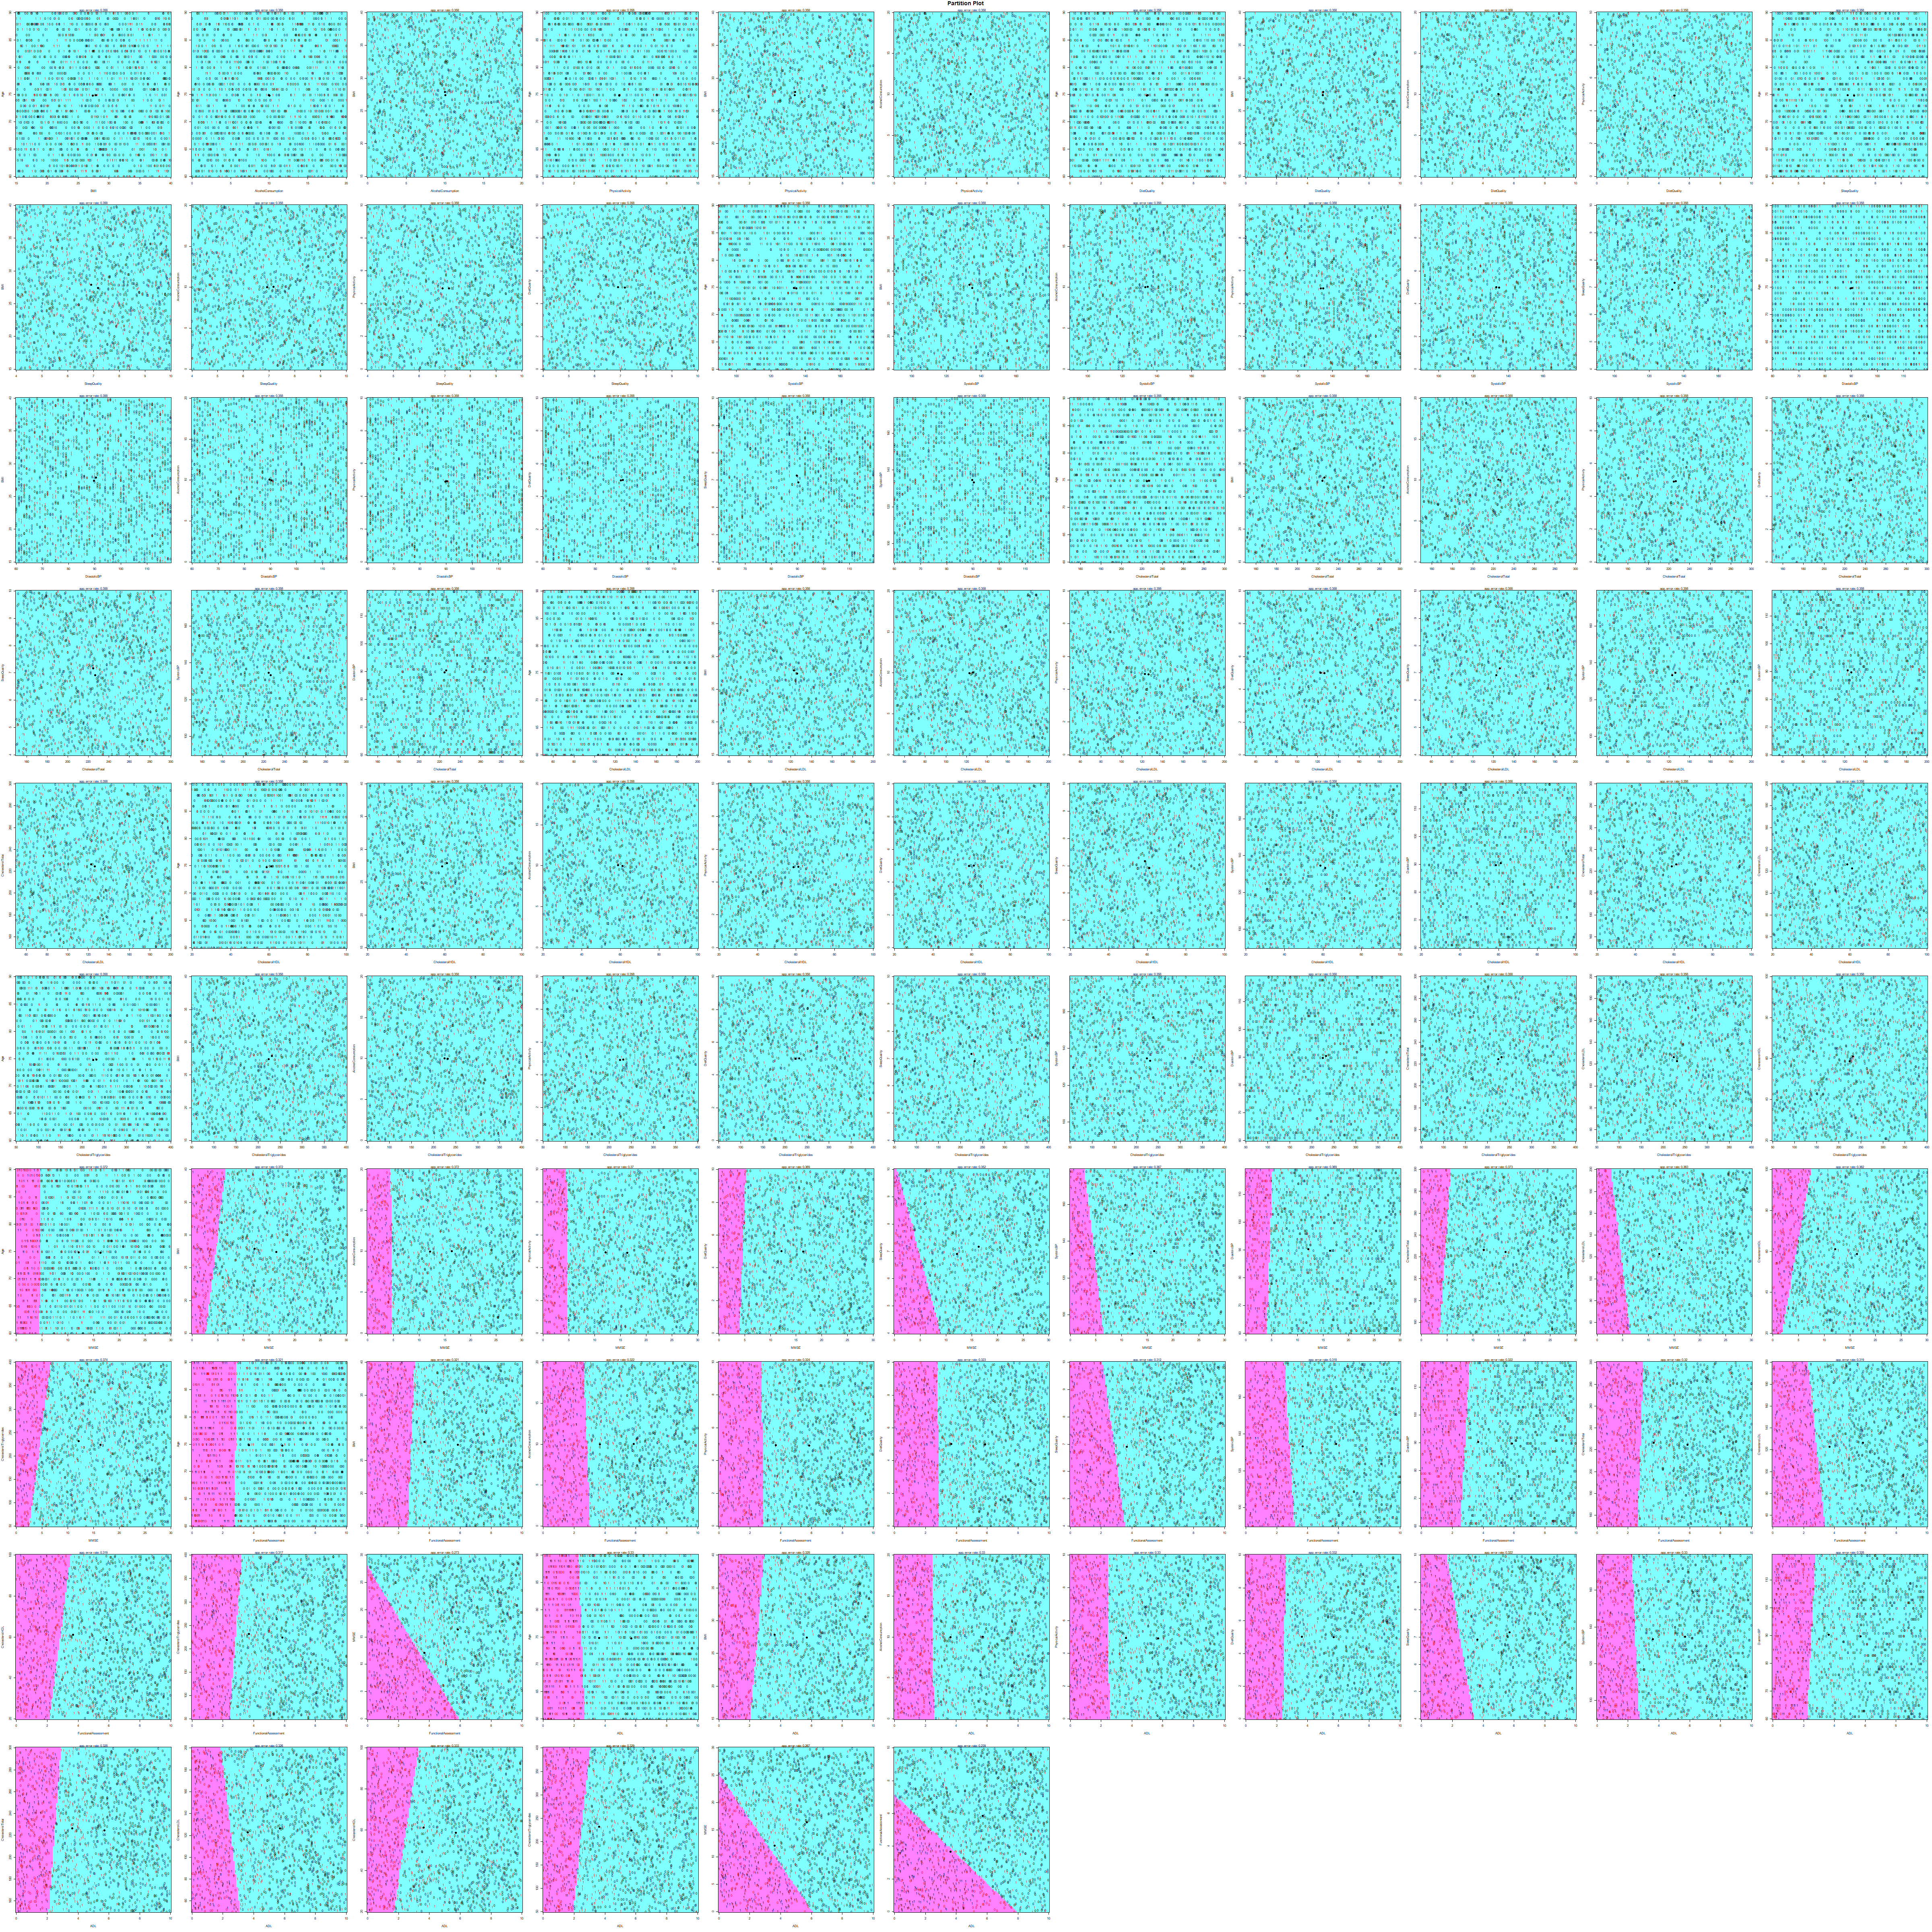
\includegraphics[width = 0.8\textwidth]{PartitionLDA.png}
\end{center}

The figure displays that among the 105 possible partition plots for LDA, only 39 pairs show clear separation between AD and Non-AD patients. Notably, all of these 39 plots include at least one the following
variables: MMSE, Functional Assessment, or ADL. This suggests that these three variables may hold the strongest discriminative power in distinguishing the two groups, as they consistently contribute to visible
class separation. In contrast, the remaining variables, when analyzed in pairs without MMSE, Functional Assessment, and ADL, do not provide distinct visual partitions, implying that these lack stronger linear 
discriminative ability on their own. 

\noindent
\textbf{Figure 8}\\
\textit{Complete Quadratic Class Discrimination of AD and Non-AD Patients}
\begin{center}
    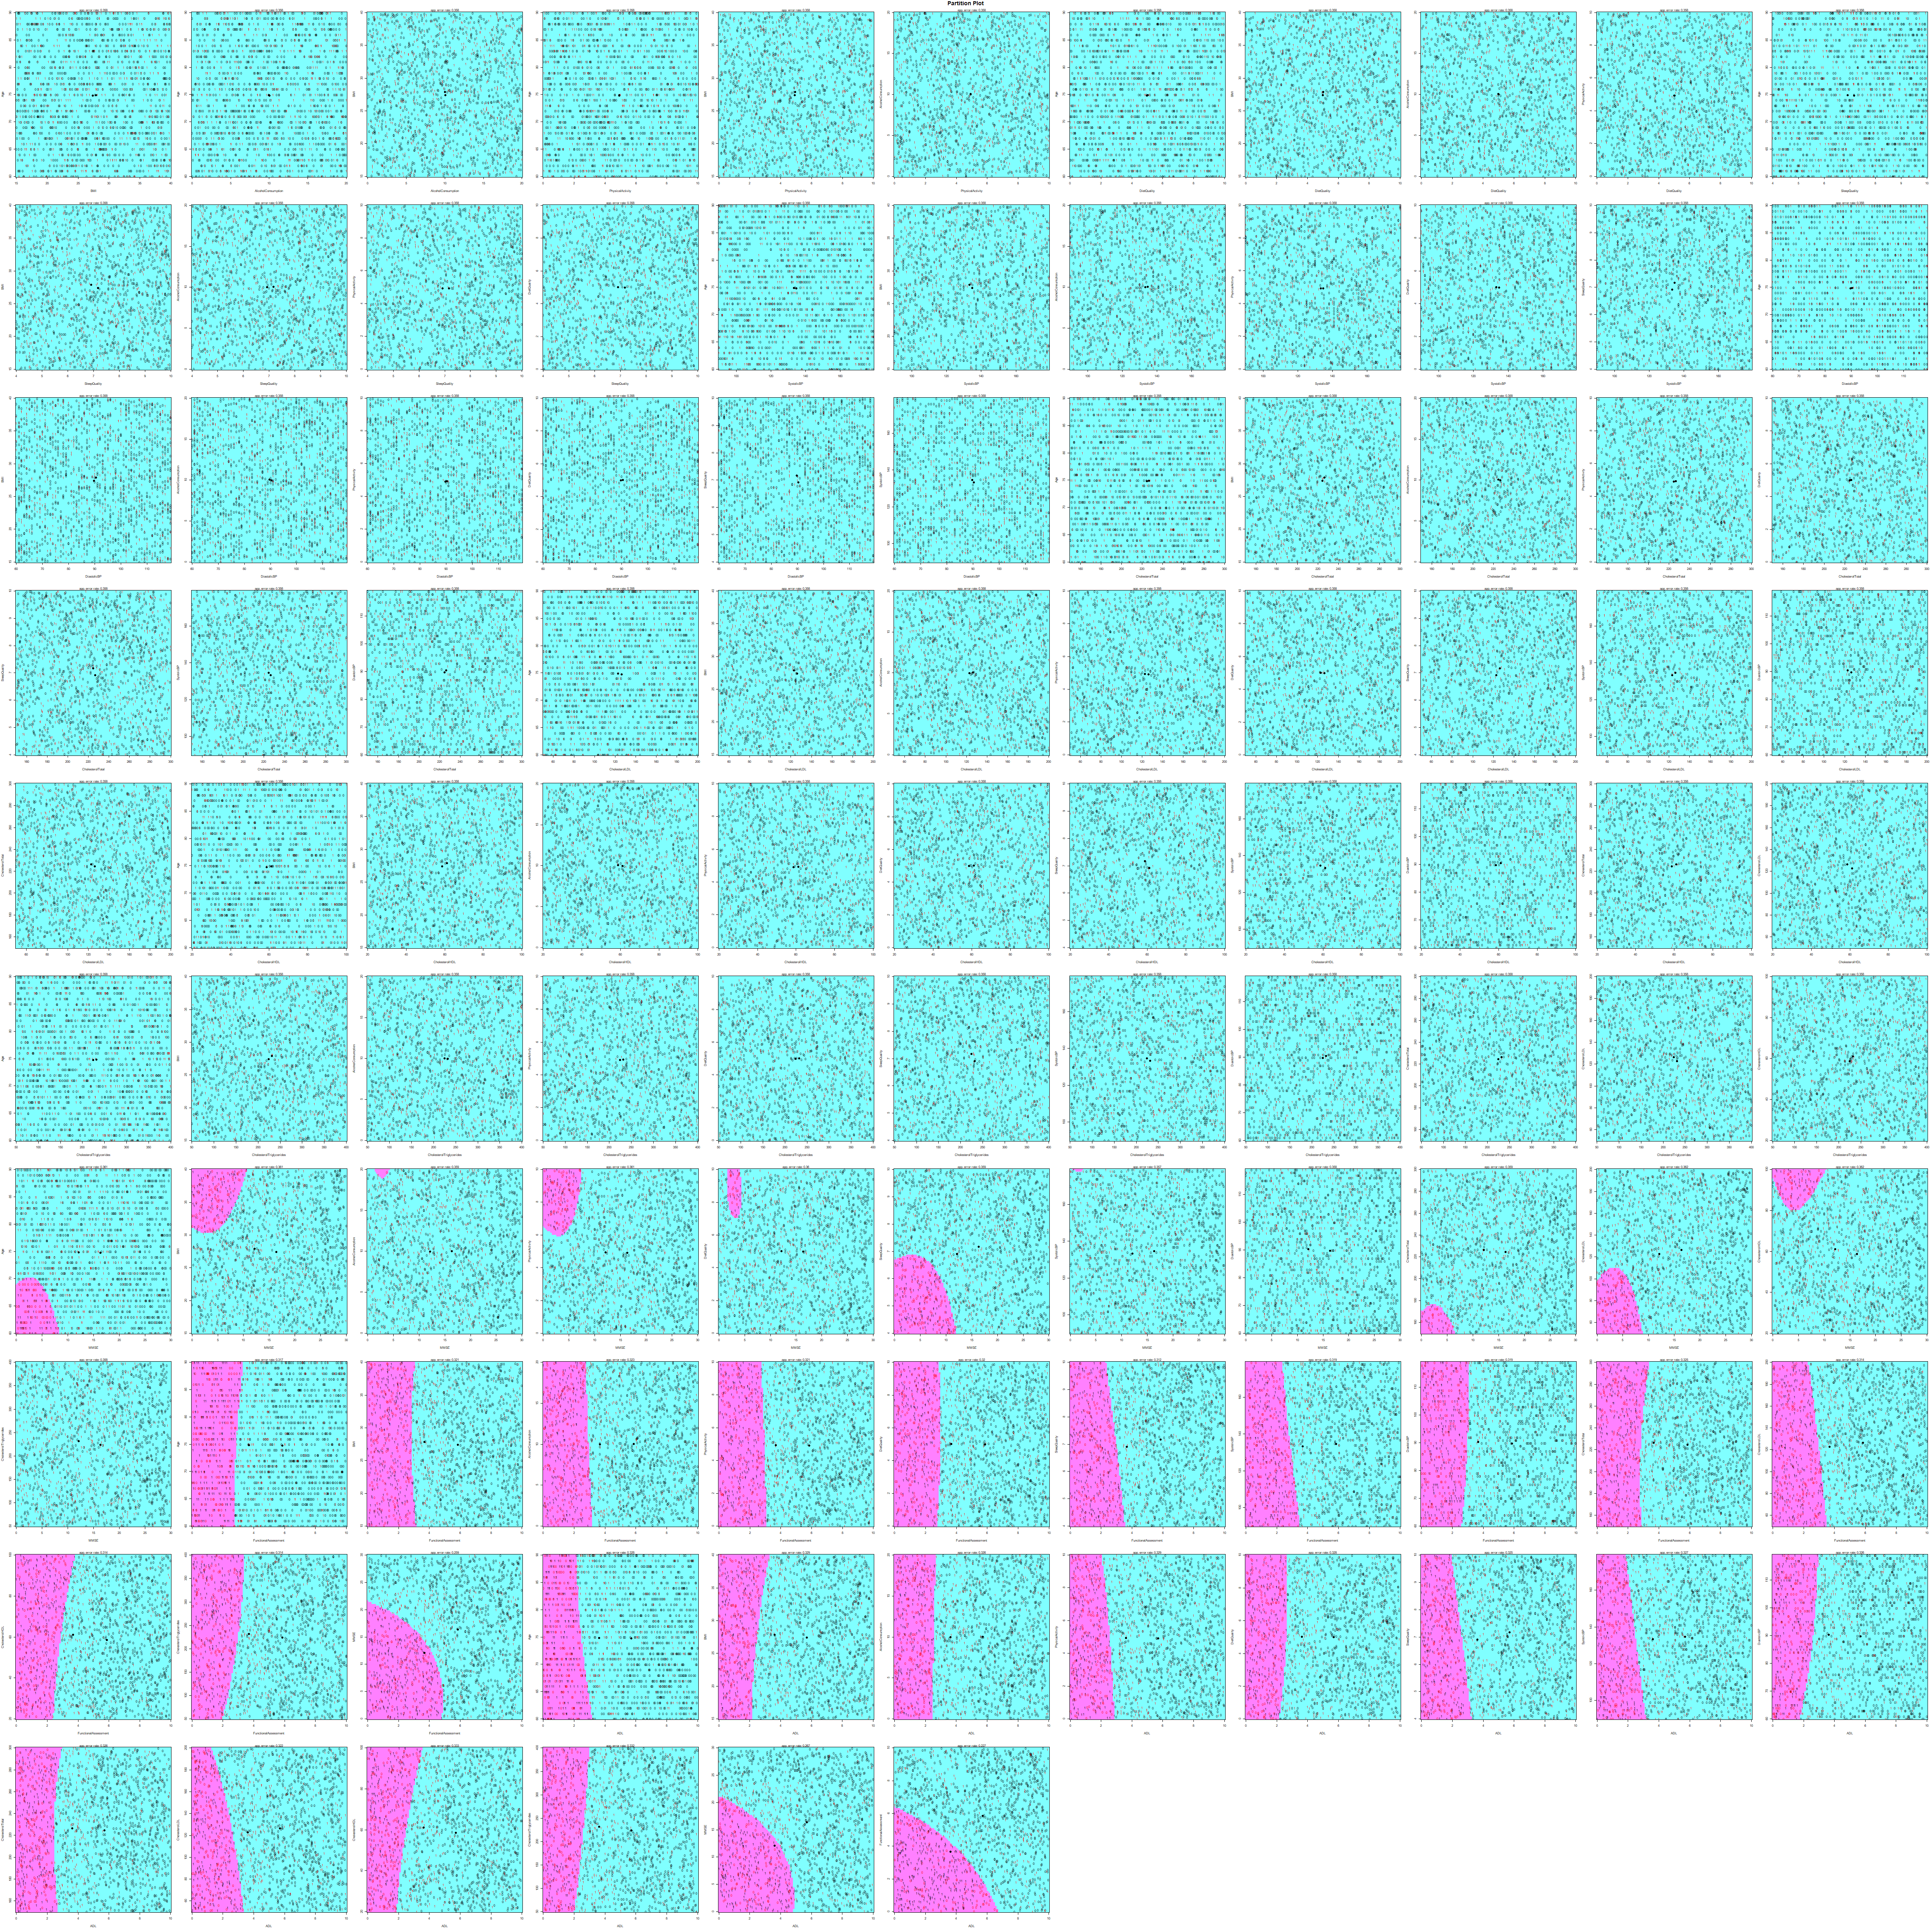
\includegraphics[width = 0.8\textwidth]{PartitionQDA.png}
\end{center}

On the other hand, the figure above shows the 105 possible partition plots for QDA, and almost similar to LDA, only 38 pairs were able to provide distinct separation between diagnosed AD and Non-AD. Specifically, the pairing of MMSE and Diastolic Blood 
Pressure did not show any partition in QDA, as compared to LDA. Through visual inspection, the pairs that include MMSE could only partition smaller and limited regions. This could mean that its effect on distinguishing AD and Non-AD patients may not be consistent 
across all values through QDA. Instead, its discriminative ability might be more pronounced in specific subgroups or at extreme values, which in this case are low MMSE scores, rather than across the entire scale range. This simply means that while it's relevant in distinguishing, 
MMSE might not be a standalone predictor in nonlinear classification method. 

\subsubsection{RFE-Reduced Linear and Quadratic Discriminant Models}
\textbf{Figure 9}\\
\textit{Root Mean Squared Error Comparison of Increasing Number of Features}
\begin{center}
    \includegraphics[width = 0.8\textwidth]{Required Number of Features.png}
\end{center}

To determine the optimal number of features for discriminating between AD and Non-AD patients, as shown in figure 9, the error metrics of each model is evaluated as the number of features increases. A significant decline in error is observed after testing the model with three features. Beyond this, the model's error
stabilized, with values consistently close to 0.35. Thus, the reduced model for both LDA and QDA should only have at least three features as predictors to achieve lower error measures and stability. 

\noindent
\textbf{Figure 10} \\
\textit{Recursive Feature Comparison by Importance}
\begin{center}
    \includegraphics[width = 0.8\textwidth]{RFE Feature Selection.png}
\end{center}

Using the same caret algorithm, variable importance is determined using RFE. In figure 10, MMSE, Functional Assessments, and ADL play a significant role in differentiating AD and Non-AD patients, which is consistent with the findings from the density distributions of cognitive and functional assessment and from the complete model of the previous 
discussions. Aside from these three, other variables have no substantial contribution to the distinction of AD and Non-AD patients as evident on the graph. 

\noindent
\textbf{Figure 11} \\
\textit{RFE-Reduced Linear Class Discrimination Model of AD and Non-AD Patients}
\begin{center}
    \includegraphics[width = 0.8\textwidth]{LDA_RFE.png}
\end{center}

Consequently, using the reduced number of features and the variables with the highest importance in figures 9 and 10, respectively, figure 11 displays the linear discrimination of AD patients and Non-AD patients. Compared to the full model, all partition pairs in the RFE-reduced linear model 
captured the distinct separation between the two classes. However, the combination of pairings was reduced to three. 

\noindent
\textbf{Figure 12} \\ 
\textit{RFE-Reduced Quadratic Class Discrimination Model of AD and Non-AD Patients}
\begin{center}
    \includegraphics[width = 0.8\textwidth]{QDA_RFE.png}
\end{center}

Similar trends can be observed in the quadratic discrimination of AD patients and Non-AD patients. All partition pairs in the reduced quadratic model captured the nonlinear distinct separation between the two classes. However, consistently, the combination of pairings was reduced to three. 

\subsubsection{Lasso Regression-Reduced Linear and Quadratic Discriminant Models}
\textbf{Figure 13} \\ 
\textit{Lambda Regularization by Feature Coefficients}
\begin{center}
    \includegraphics[width = 0.8\textwidth]{Coefficient vs Log Lambda.png}
\end{center}

The logarithm of lambda controls the regularization strength of the coefficients for feature reduction. As the value of lambda increases, more coefficients shrink towards zero which indicates that more features are being penalized by the model. Based on the graph, along lambda values of -5 to -3, the model 
achieves the best trade-off between coefficient shrinkage and performance. 

\noindent
\textbf{Figure 14}\\
\textit{Binomial Deviance and Logarithmic Lambda}
\begin{center}
    \includegraphics[width = 0.8\textwidth]{Binomial Deviance vs Log Lambda.png}
\end{center}

Upon cross-validated, figure 9 displays the error rate of the lambda values as it increases. The red dot are the mean coefficients and vertical lines are its error rates. As the lambda value increases the error rate is also increasing, shrinking the coefficients down to zero. 

\noindent
\textbf{Figure 15}\\
\textit{Feature Importance based on the Optimal Lambda}
\begin{center}
    \includegraphics[width = 0.8\textwidth]{Lasso Feature Selection.png}
\end{center}

Thus, based on the optimal lambda from the lasso regression, ADL, Functional Assessments, MMSE, and Sleep Quality were the top four contributors for discriminating AD patients and Non-AD patients. 

\noindent
\textbf{Figure 16} \\
\textit{Lasso-Reduced Linear Class Discrimination of AD and Non-AD Patients}
\begin{center}
    \includegraphics[width = 0.8\textwidth]{Lasso_Reduced_LDA.png}
\end{center}

Consequently, the feature reduction using lasso regression shrunk the diagnosis equation down to four predictors: ADL, Functional Assessments, MMSE, and Sleep Quality. It produced six pairs of partition plot which successfully classified Ad patients with Non-AD patients given by the existing
separation line between the two classes. Comparably, features involving Functional Assessments, ADL, and MMSE linearly discriminates AD patients to Non-AD patients by a larger region compared to the involvement of Sleep Quality. 

\newpage
\noindent
\textbf{Figure 17} \\
\textit{Lasso-Reduced Quadratic Class Discrimination of AD and Non-AD Patients}
\begin{center}
    \includegraphics[width = 0.8\textwidth]{Partimat_QDA_Lasso.png}
\end{center}

The effect of the reduction remained consistent with the quadratic approach, with the primary difference being that the separation line was curved rather than linear. However, the separation lines between Functional Assessments and Sleep Quality, as well as between ADL and Sleep Quality, remained linear. 
Additionally, the region of separation between MMSE and Sleep Quality contracted compared to the linear approach.

\newpage
\subsection{Classification Metrics Comparisons of LDA and QDA Models}
\textbf{Figure 18} \\
\textit{Model Accuracies Across 10-Folds}
\begin{center}
    \includegraphics[width = 0.8\textwidth]{Accuracy_Line_plots.png}
\end{center}

Each discriminant analysis model is evaluated using accuracy measures across 10 folds, using 8:2 training-to-testing ratio in each fold. As shown in figure 18, Lasso Regression-Reduced QDA model achieves the highest accuracy at 6th fold, 
indicating its strong performance in distinguishing between AD and Non-AD patients. Conversely, the Lasso Regression-Reduced LDA records the lowest accuracy at 9th fold, suggesting higher variability in its classification performance. 

The overall trend implies that Lasso Regression-Reduced QDA consistently captures membership classification with greater accuracy, making it more reliable choice for distinguishing AD from Non-AD patients compared to other discriminant models. 

\newpage
\noindent
\textbf{Table 3}\\
\textit{Classification Metrics by Discriminant Model}
\begin{center}
    \begin{tabular}{lcccccc}
        \hline
        \textit{Model} & \textit{Accuracy} & \textit{Specificity} & \textit{Sensitivity} & \textit{F1-Score} & \textit{NIR} & \textit{p-value} \\
        \hline
        Complete LDA & 0.7712 & 0.8172 & 0.7248 & 0.6972 & 0.6627 & \(\textless 0.01\) \\
        Complete QDA & 0.7689 & 0.8000 & 0.8683 & 0.7684 & 0.6627 & \(\textless 0.01\) \\
        RFE LDA & 0.7594 & 0.5804 & 0.8505 & 0.8241 & 0.6627 & \(\textless 0.01\) \\
        RFE QDA & 0.7830 & 0.5804 & 0.8861 & 0.8441 & 0.6627 & \(\textless 0.01\) \\
        Lasso LDA & 0.7712 & 0.6014 & 0.8577 & 0.8325 & 0.6627 & \(\textless 0.1\) \\ 
        Lasso QDA & 0.7854 & 0.5844 & 0.8826 & 0.8450 & 0.6627 & \(\textless 0.01\) \\
        \hline
    \end{tabular}
\end{center}

The classification results indicate that Lasso QDA and RFE QDA are the best performing models, achieving the highest average accuracies of 78.54\% and 78.30\%, respectively, and F1-scores of 
84.50\% and 84.41\%, respectively. Both models also exhibit high sensitivity, with Lasso QDA (88.25\%) and RFE QDA (88.61\%), suggesting they are particularly effective at identifying positive cases. 
However, their specificity remains relatively low with both models around 58\%, which indicates a tendency to misclassify negative cases. In contrast, Complete LDA has the highest specificity of 81.72\%, making 
it better suited for correctly identifying negative cases, but at the cost of lower sensitivity of 72.48\%. The statistical significance of all models suggests that they significantly outperform NIR of 66.27\%. 

Moreover, the classification results also revealed that QDA-based models perform better overall, particularly when combined with Lasso Regression and RFE for feature reduction techniques. 


\newpage
\section{CHAPTER V \\ CONCLUSION AND RECOMMENDATION}
\noindent 

This chapter covers the summary from the results of the study, and the conclusions of the researchers drawn based on the results. Recommendations for the study are also discussed in this section. 

\subsection{Summary of Findings}
\noindent

The probability density plots of each features of AD revealed significant differences on the cognitive and functional assessment scores of AD and Non-AD patients. AD patients showed lower functional abilities and 
severe cognitive impairment based on their respective test results. However, both lifestyle factors and clinical measurement indicators remained to be consistent between the two groups. The three features of Cognitive and 
Functional Assessments became the substantial identifier for AD and Non-AD discrimination. For the full models of both LDA and QDA, the three variables: MMSE, FunctionalAssessment, and ADL provided distinct partitions across the 
105 combination of features. Consequently, the features are reduced using both RFE and Lasso Regression, MMSE, FunctionalAssessment, and ADL remained to have the highest importance for predicting AD patients. 

The general objective of the study is to determine an optimal model that can predict AD and Non-AD classification using both LDA and QDA models. Through 10-Fold Cross Validation of Accuracy measures, Lasso-Regression with the optimal lambda value achieved
the highest accuracy at its 6th fold, the highest record among all models and among all folds. Using a confusion matrix to determine classification metrics of all the models, Lasso Regression-Reduced QDA achieved the highest in accuracy, sensitivity and F1 score. 
It reveals that the Lasso Regression Reduced QDA measures the proportion of actual positive cases in acceptable thresholds even when the positive and negative classes are not evenly distributed. 

Overall, for Alzheimer's disease prediction, Quadratic models in general achieved better performances compared to Linear Models. 

\subsection{Conclusion}
Based on the findings of the study, these conclusions are drawn: 
\begin{itemize}
    \item The study concludes that Cognitive and Functional Assessment Scores are key indicators of Alzheimer's Disease. Specifically, low scores in MMSE, Functional Assessment, and ADL are strongly associated with the potential development of Alzheimer's Disease.
    \item The study finds that Quadratic Discriminant Models have the optimal accuracy in predicting Alzheimer's occurrence. 
\end{itemize}

\subsection{Recommendations}
For the improvement in the fields of discriminant models and Alzheimer's disease prediction, the researchers recommend the following: 
\begin{itemize}
    \item The synthetic nature of the dataset prevents the generalizability of the results. Using a more realistic data may improve AD and Non-AD classification using the other feature. 
    \item Aside from the cognitive and functional assessment scores as main identifier of AD, adding numerical variables based on patient lifestyle and other clinical measurements may enrich the model complexity and may reveal hidden relationships. 
    \item This study classifies the dependent variable based on patient diagnosis (presence or absence of the disease). Extending LDA and QDA to multi-category variables, like Alzheimer's stages, may improve classification accuracy. 
\end{itemize}

\newpage
\raggedleft
\defbibheading{bibliography}[\refname]{\section*{\raggedleft#1}}
\printbibliography

\end{document}